\chapter{Numerical experiments} \label{chap:NumExp}
This chapter presents some numerical experiments in order to illustrate the potential advantages of considering inexact schemes in the SGP method.
We will discuss inexactness associated with both the projection onto the feasible set and the line search procedure.

Given $A$ and $B$ two $m\times n$ matrices, with $m\geq n$, and $c\in\R$, we consider the matrix function $f:\R^{n\times n}\to\R$ given by:
\begin{equation}\label{objfun}
	f(X):=\ds\frac{1}{2}\|AX-B\|^2_F + \sum_{i=1}^{n-1} \left[ c \left( X_{i+1,i+1}-X_{i,i}^2 \right)^2 + (1-X_{i,i})^2   \right],
\end{equation}
which combines a least squares term with a Rosenbrock-type function.
Throughout this section, $X_{i,j}$ stands for the $ij$-element of the matrix $X$ and $\|\cdot\|_F$ denotes the Frobenius matrix norm, i.e., $\|A\|_F:=\sqrt{\langle A,A \rangle}$ where the inner product is given by $\langle A,B \rangle = \tr(A^TB)$.
The test problems consist of minimizing $f$ in \eqref{objfun} subject to two different feasible sets, as described below.
We point out that interesting applications in many areas emerge as constrained least squares matrix problems, see \cite{BirginMartinezRaydan2003} and references therein.
In turn, the Rosenbrock term was added in order to make the problems more challenging.

\begin{description}
	\item[{\bf Problem~I:}]
		\begin{equation*} \label{sdd}
			\begin{array}{cl}
				\ds\min     & f(X)           \\
				\mbox{s.t.} & X \in SDD^+,   \\
				            & L\leq X\leq U,
			\end{array}
		\end{equation*}
		where $SDD^+$ is the cone of symmetric and diagonally dominant real matrices with positive diagonal, i.e.,
		$$SDD^+ :=\{X\in\R^{n\times n}\mid X=X^T, \; X_{i,i}\geq \ds\sum_{j\neq i}|X_{i,j}| \; \forall i\},$$
		$L$ and $U$ are given $n\times n$ matrices, and  $L\leq X\leq U$ means that $L_{i,j} \leq X_{i,j} \leq U_{i,j}$ for all $i,j$.
		The feasible set of Problem I was considered, for example, in the numerical tests of \cite{BirginMartinezRaydan2003}.

	\item[{\bf Problem~II:}]
		\begin{equation*} \label{spec}
			\begin{array}{cl}
				\ds\min     & f(X)                  \\
				\mbox{s.t.} & X \in \mathbb{S}^n_+, \\
				            & \tr(X)=1,
			\end{array}
		\end{equation*}
		where $\mathbb{S}^n_+$ is the cone of symmetric and positive semidefinite real matrices and $\tr(X)$ denotes the trace of $X$.
		The feasible set of Problem II was known as {\it spectrahedron} and appears in several interesting applications see, for example, \cite{allen2017linear,douglasprojected} and references therein.
\end{description}

%For future reference, we will denote the feasible sets of Problems A and B by $C_A$ and $C_B$, respectively. It is easy to see that $C_A$ is  a closed and convex set and $C_B$ is  a compact and convex set. We notice that Problems A and B can be seen as particular instances of the problem~\eqref{eq:OptP} in which the number of variables is $(n^2+n)/2$.

It is easy to see that the feasible set of Problem~I is a closed and convex set and the feasible set of Problem~II is  a compact and convex set.
As discussed in Section~\ref{sec:pcip}, the Dykstra's alternating algorithm and the Frank-Wolfe algorithm can be used to calculate inexact projections. The choice of the most appropriate method depends on the structure of the feasible set under consideration.
For Problem~I, we used the Dykstra's algorithm described in \cite{BirginMartinezRaydan2003}, see also \cite{dykstraSDD}. In this case, $SDD^+=\ds\cap_{i=1}^n SDD^+_i$, where
$$SDD^+_i :=\{X\in\R^{n\times n}\mid X=X^T, \; X_{i,i}\geq \ds\sum_{j\neq i}|X_{i,j}| \} \; \mbox{for all} \; i=1,\ldots,n,$$
and the projection of a given $Z\in\R^{n\times n}$ onto $SDD^+$ consists of cycles of projections onto the convex sets $SDD^+_i$.
Here an iteration of the Dykstra's algorithm should be understood as a complete cycle of projections onto all $SDD^+_i $ sets and onto the box $\{X\in\R^{n\times n}\mid L\leq X\leq U\}$.
Recall that this scheme provides an inexact projection as in Definition~\ref{def:InexactM}.
%
Now consider Problem~II. It is well known that calculating an exact projection onto the spectrahedron (i.e., onto the feasible set of Problem~II) requires a complete spectral decomposition, which can be prohibitive specially in the large scale case. In contrast, the computational cost of an iteration of the Frank-Wolfe algorithm described in Algorithm~\ref{Alg:CondG} is associated by an extreme eigenpair computation, see, for example, \cite{Jaggi2013}. Unfortunately, despite its low cost per-iteration, the Frank-Wolfe algorithm suffers from a slow convergence rate.
Thus, we considered a variant of the Frank-Wolfe algorithm proposed in \cite{allen2017linear}, which improves the convergence rate and the total time complexity of the classical Frank-Wolfe method. This algorithm specialized for the projection problem over the spectrahedron is carefully described in \cite{aguiar2021inexact}.
Without attempting to go into details, it replaces the top eigenpair computation in Frank-Wolfe with a top-$p$ (with $p\ll n$) eigenpair computation, where $p$ is an algorithmic parameter automatically selected.
The total number of computed eigenpairs can be used to measure the computational effort to calculate projections.
We recall that a Frank-Wolfe type scheme provides an inexact projection as in Definition~\ref{def:InexactProjC}.


We notice that Problems~I and II can be seen as particular instances of the problem~\eqref{eq:OptP} in which the number of variables is $(n^2+n)/2$. This mean that they can be solved by using Algorithm~\ref{Alg:GeneralSeach}.
We are especially interested in the spectral gradient version \cite{BirginMartinezRaydan2003,spgsiam} of the SGP method, which is often associated with large-scale problems \cite{JSSv060i03}. For this, we implemented Algorithm~\ref{Alg:GeneralSeach} considering $D_k:=I$ for all $k$, $\alpha_0 := \min(\alpha_{\max}, \max(\alpha_{\min}, 1/ \| \nabla f(x^0) \|))$ and, for $k>0$,
\begin{equation*}\label{spg}
	\alpha_k:=\left\{\begin{array}{ll}
		\ds\min (\alpha_{\max},\max (\alpha_{\min},\langle s^k,s^k\rangle/\langle s^k,y^k\rangle)), & \mbox{if} \; \langle s^k,y^k\rangle > 0 \\
		\alpha_{\max},                                                                              & \mbox{otherwise},
	\end{array}\right.
\end{equation*}
where $s^k:=X^k - X^{k-1}$, $y^k:=\nabla f(X^k) - \nabla f(X^{k-1})$, $\alpha_{\min}=10^{-10}$, and $\alpha_{\max}=10^{10}$.
We set $\sigma = 10^{ -4}$, $\underline\tau=0.1$, $\bar\tau=0.9$, $\mu=1$ and $\nu_0=0$. Parameter $\delta_{\min}$ was chosen according to the line search used (see Section~\ref{chap:SGM}), while parameter $\zeta_{\min}$ depends on the inexact projection scheme considered.

In the line search scheme (Step~2 of Algorithm~\ref{Alg:GeneralSeach}), if a step size $\tau_{\textrm{trial}}$  is not accepted, then $\tau_{\textrm{new}}$ is calculated using one-dimensional quadratic interpolation employing the safeguard $\tau_{\textrm{new}}\gets \tau_{\textrm{trial}}/2$  when the minimum of the one-dimensional quadratic lies outside $[\underline\omega \tau_{\textrm{trial}}, \bar\omega \tau_{\textrm{trial}} ]$, see, for example,  \cite[Section 3.5]{nocedal2006numerical}.
Concerning the stopping criterion, all runs were stopped at an iterate $X^k$ declaring convergence if
$$\ds \max_{i,j} (|X^k_{i,j}-W^k_{i,j}| )\leq 10^{-6},$$
where $W^k$ is as in \eqref{eq:PInexArm}.
Our codes are written in Matlab and are freely available at \url{https://github.com/maxlemes/SGP}. All experiments were run on a macOS 10.15.7 with 3.7GHz Intel Core i5 processor and 8GB of RAM.
%%%%%%%%%%%%%%%%%%%%%%%%%%%%%%%%%%%%%%
\section{Influence of the inexact projection} \label{sec:forcing}
We begin the numerical experiments by checking the influence of the forcing parameters that control the degree of inexactness of the projections in the performance of the  method. In this first battery of tests, we used Armijo line searches, see Section~\ref{chap:SGM}.

We generated 10 instances of Problem~I using $n=100$, $m=200$, and $c=10$. The matrices $A$ and $B$ were randomly generated with elements belonging to $[-1,1]$. We set $L\equiv 0$ and $U\equiv \infty$ as in \cite{BirginMartinezRaydan2003}. For each instance, the starting point $X^0$ was randomly generated with elements belonging to $[0,1]$, then it was redefined as $(X^0 + (X^0)^T )/2$ and its diagonal elements were again redefined as $2\sum_{j\neq i}^n X_{i,j}$, ensuring a feasible starting point. Figure~\ref{SDD} shows the average number of iterations,  the average number of Dykstra’s iterations, and the average  CPU time in seconds needed to reach the solution for different choices of $\zeta_k$, namely, $\zeta_k=0.99$, $0.9$, $0.8$, $0.7$, $0.6$, $0.5$, $0.4$, $0.3$, $0.2$, and $0.1$ for all $k$.
Remember that {\it smaller values} of  $\zeta_k$ imply {\it more inexact} projections. As expected, the number of iterations  tended to increase as $\zeta_k$ decreased, see  Figure~\ref{SDD}(a).
On the other hand, the computational cost of an outer iteration (which can be measured by the number of Dykstra’s iterations) tends to decrease when considering smaller values of $\zeta_k$.
This suggests a trade-off, controlled by parameter $\zeta_k$, between the number and the cost per iteration.
Figure~\ref{SDD}(b) shows that values for $\zeta_k$ close to 0.8 showed better results, which is in line with the experiments reported in \cite{BirginMartinezRaydan2003}.
Finally, as can be seen in Figure~\ref{SDD}(c), the CPU time was shown to be directly proportional to the number Dykstra’s iterations.
\begin{figure}[H]\centering
	\begin{tabular}{ccc}
		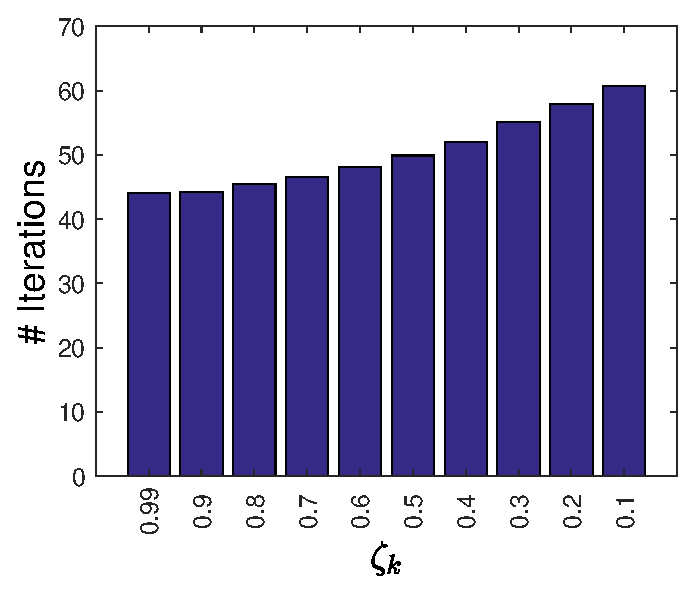
\includegraphics[scale=\myscale]{figures/SDDit} & 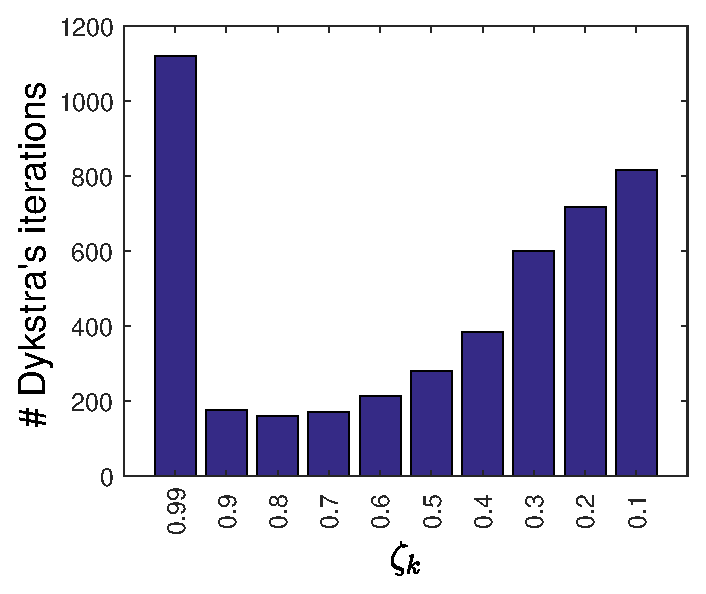
\includegraphics[scale=\myscale]{figures/SDDDIT} & 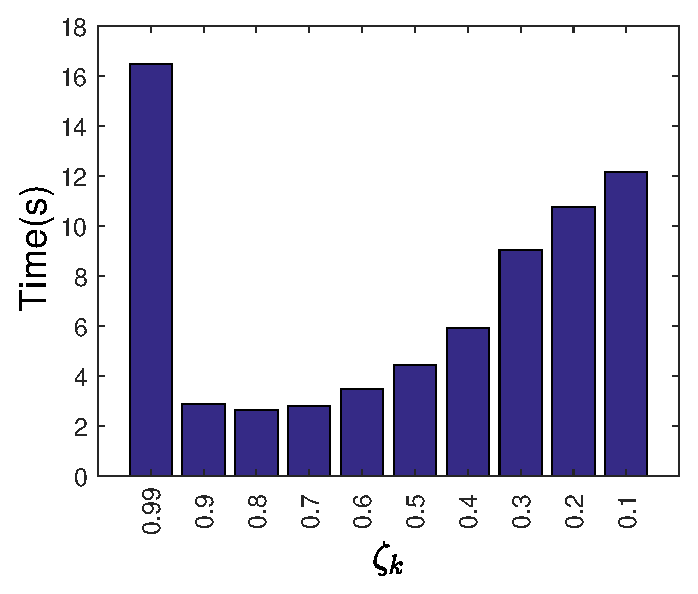
\includegraphics[scale=\myscale]{figures/SDDtime} \\
		(a)                                             & (b)                                              & (c)                                               \\
	\end{tabular}
	\caption[Results for 10 instances of Problem I]{Results for 10 instances of Problem I using $n=100$, $m=200$, and $c=10$. Average number of: (a) iterations; (b) Dykstra’s iterations; (c)  CPU time in seconds needed to reach the solution for different choices of $\zeta_k$.}
	\label{SDD}
\end{figure}

Although Algorithm~\ref{Alg:GeneralSeach} is given only in terms of parameter $\zeta_k$, we will directly consider parameter $\gamma_k$ for Problem~II in which inexact projections are computed according to Definition~\ref{def:InexactProjC}. We randomly generated 10 instances of Problem~II with $n=800$, $m=1000$, and $c=100$. Matrices $A$ and $B$ were obtained similarly to Problem~I. In turn, a starting point $X^0$ was randomly generated with elements in the interval $[-1,1]$, then it was redefined to be $X^0  (X^0)^T/\tr(X^0  (X^0)^T)$, resulting in a feasible initial guess.
Figure~\ref{Spec} shows the average number of iterations,  the average number of computed eigenpairs, and the average  CPU time in seconds needed to reach the solution for different constant choices of $\gamma_k$ ranging from $10^{-8}$ to $0.4999$. Now, {\it higher values} of $\gamma_k$ imply {\it more inexact} projections. Note that for appropriate choices of $\zeta_k$, the adopted values of $\gamma_k$ fulfill Assumption A1 of Section~\ref{Sec:FullConvRes}. Concerning the number of iterations, as can be seen in Figure~\ref{Spec}(a),  the algorithm was not very sensitive to the choice of parameter $\gamma_k$. Hence, since higher values of $\gamma_k$ imply cheaper iterations, the number of computed eigenpairs and the CPU time showed to be inversely proportional to $\gamma_k$, see Figures~\ref{Spec}(b)--(c). Thus, our experiments suggest that the best value for $\gamma_k$ seems to be $0.4999$.

\begin{figure}[H]\centering
	\begin{tabular}{ccc}
		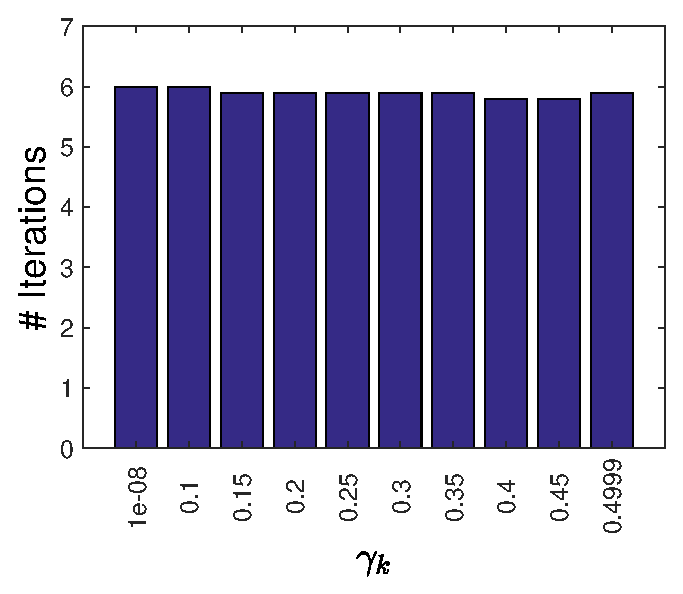
\includegraphics[scale=\myscale]{figures/Specit} & 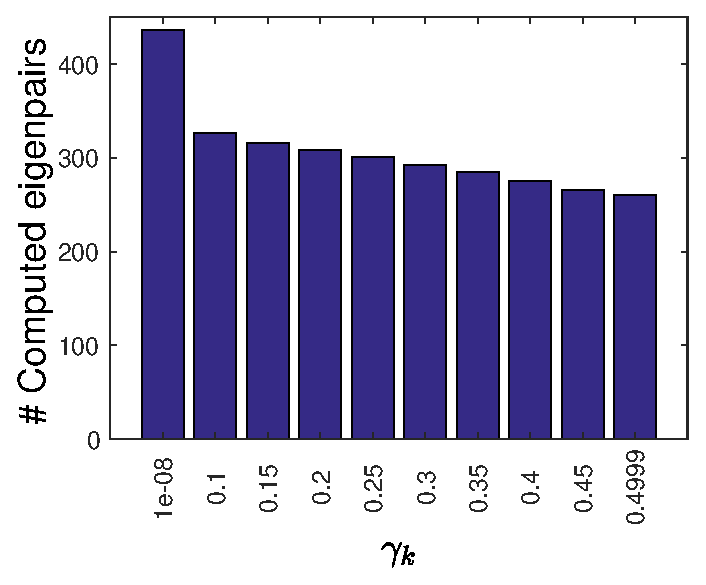
\includegraphics[scale=\myscale]{figures/SpecFWIT} & 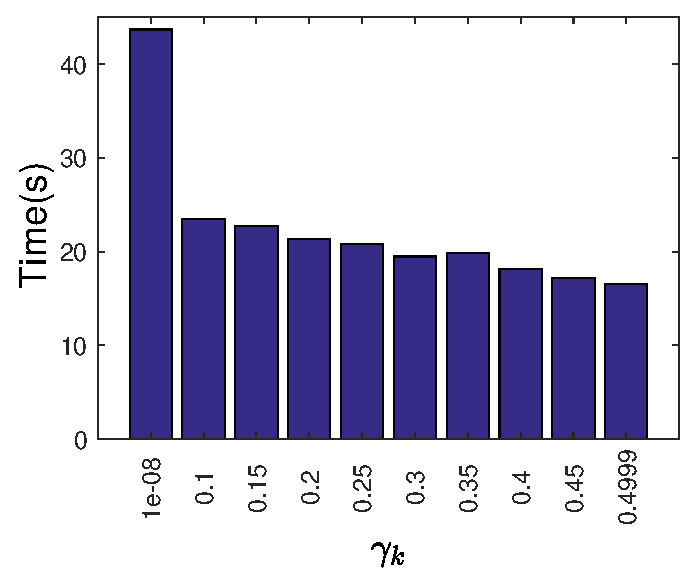
\includegraphics[scale=\myscale]{figures/Spectime} \\
		(a)                                              & (b)                                                & (c)                                                \\
	\end{tabular}
	\caption[Results for 10 instances of Problem II]{Results for 10 instances of Problem II using $n=800$, $m=1000$, and $c=100$. Average number of: (a) iterations; (b) computed eigenpairs; (c)  CPU time in seconds needed to reach the solution for different choices of $\gamma_k$.}
	\label{Spec}
\end{figure}

\section{Influence of the line search scheme}

The following experiments compare the performance of the algorithm with different strategies for computing the step sizes. We considered the Armijo, the Average-type, and the Max-type line searches discussed in Section~\ref{chap:SGM}.
Based on our numerical experience, we employed the fixed value $\eta_k=0.85$ for the Average-type line search and $M=5$ for the Max-type line search.
According to the results of the previous section, we used the fixed forcing parameters $\zeta_k=0.8$ and $\gamma_k=0.4999$ to compute inexact projections for Problems~I and II, respectively.

We randomly generated 100 instances of each problem as described in Section~\ref{sec:forcing}. The dimension of the problems and the parameter $c$ in \eqref{objfun} were also taken arbitrarily. For Problem~I, we choose $100\leq n \leq 800$ and $10\leq c \leq 50$, whereas for Problem~II, we choose $10\leq n \leq 200$ and $100\leq c \leq 1000$. In both cases, we set $m=2n$.
We compare the strategies with respect to the number of function evaluations, the number of (outer) iterations, the total computational effort to calculate projections (measured by the number of Dykstra’s iterations and computed eigenpairs for Problems~I and II, respectively), and the CPU time. The results are shown in Figures~\ref{ppSDD} and \ref{ppSpec} for Problems~I and II, respectively, using performance profiles \cite{dolan2002benchmarking}.

For Problem~I, with regard to the number of function evaluations, the algorithm with the Average-type line search was the most efficient among the tested strategies.
In a somewhat surprising way, in this set of test problems, the Armijo strategy was better than the Max-type line search, see Figure~\ref{ppSDD}(a).
On the other hand, as can be seen in Figure~\ref{ppSDD}(b), the Armijo strategy required fewer iterations than the nonmonotone strategies.
As expected, this was reflected in the number of Dykstra’s iterations and the CPU time, see Figures~\ref{ppSDD}(c)--(d).
We can conclude that, with respect to the last two criteria, the Armijo and Average-type strategies had similar and superior performances to the Max-type strategy.

Now, concerning Problem~II, Figure~\ref{ppSpec} shows that the nonmonotone strategies outperformed the Armijo strategy in all the comparative criteria considered.
Again,  the Average-type strategy seems to be superior to the Max-type strategy.

\begin{figure}[H]\centering
	\begin{tabular}{cccc}
		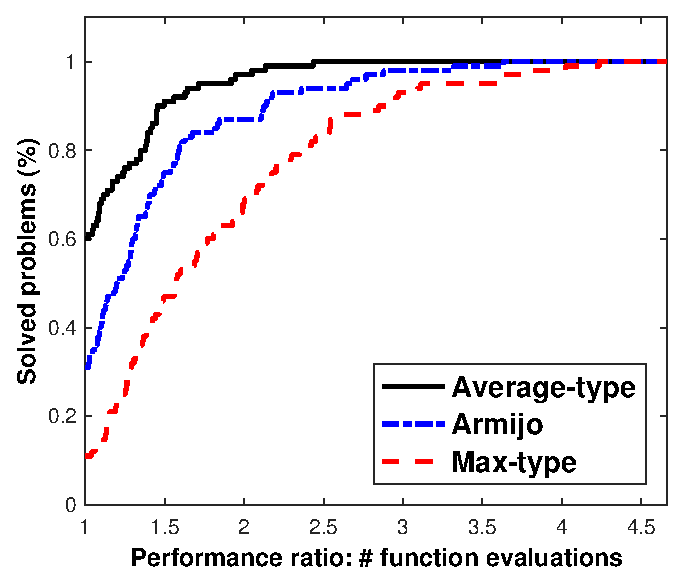
\includegraphics[scale=\myscale]{figures/ppSDDnfev} & 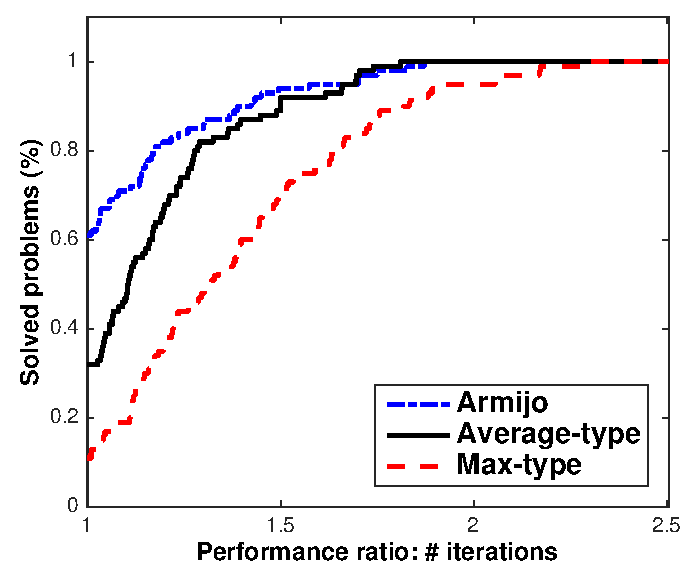
\includegraphics[scale=\myscale]{figures/ppSDDit} & 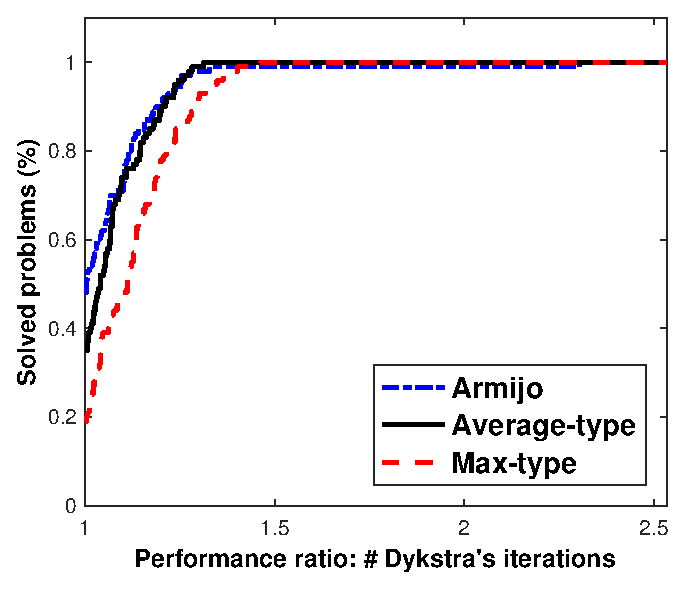
\includegraphics[scale=\myscale]{figures/ppSDDnDIT} & 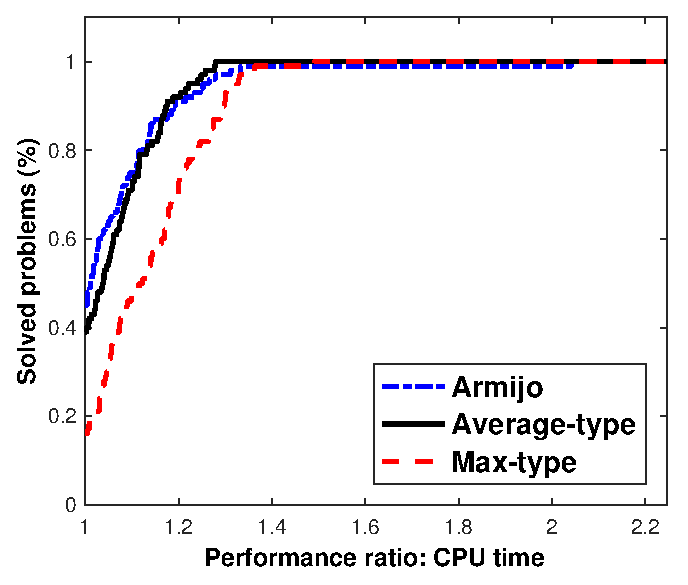
\includegraphics[scale=\myscale]{figures/ppSDDtime} \\
		(a)                                                 & (b)                                               & (c)                                                 & (d)                                                 \\
	\end{tabular}
	\caption[Performance profiles for Problem~I]{Performance profiles for Problem~I considering  Algorithm~\ref{Alg:GeneralSeach} with the Armijo, the Average-type, and the Max-type line searches strategies using as performance measurement: (a) number of function evaluations; (b) number of (outer) iterations; (c) number of Dykstra’s iterations; (d) CPU time.}
	\label{ppSDD}
\end{figure}

\begin{figure}[H]\centering
	\begin{tabular}{cccc}
		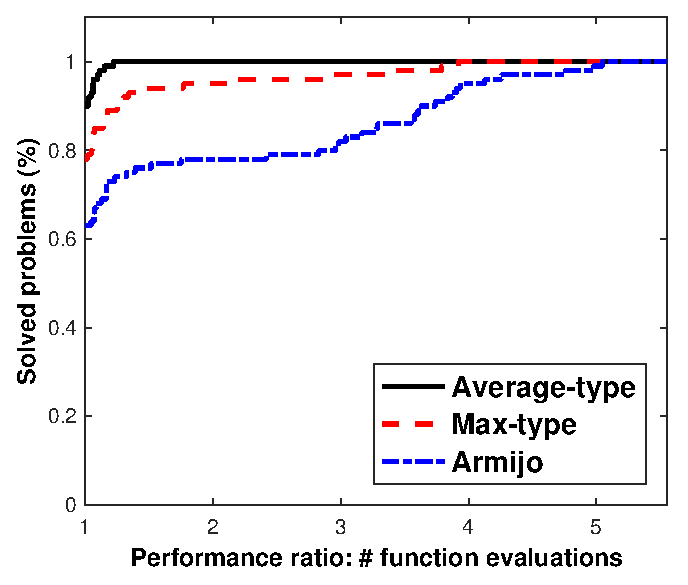
\includegraphics[scale=\myscale]{figures/ppSpecnfev} & 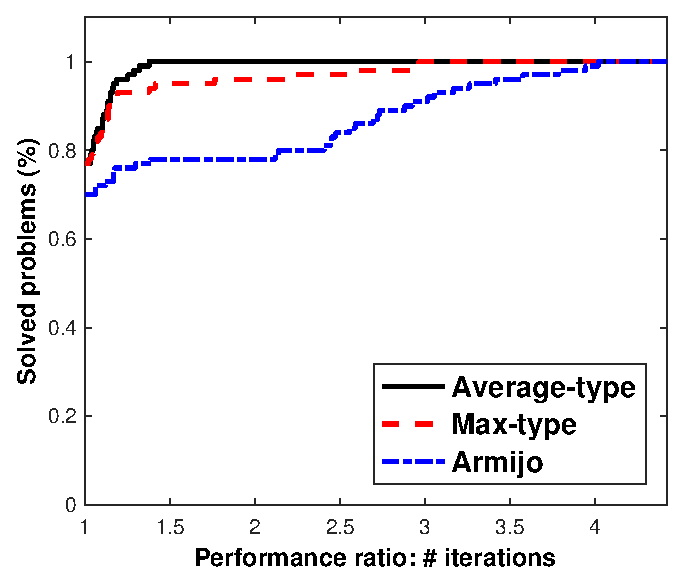
\includegraphics[scale=\myscale]{figures/ppSpecit} & 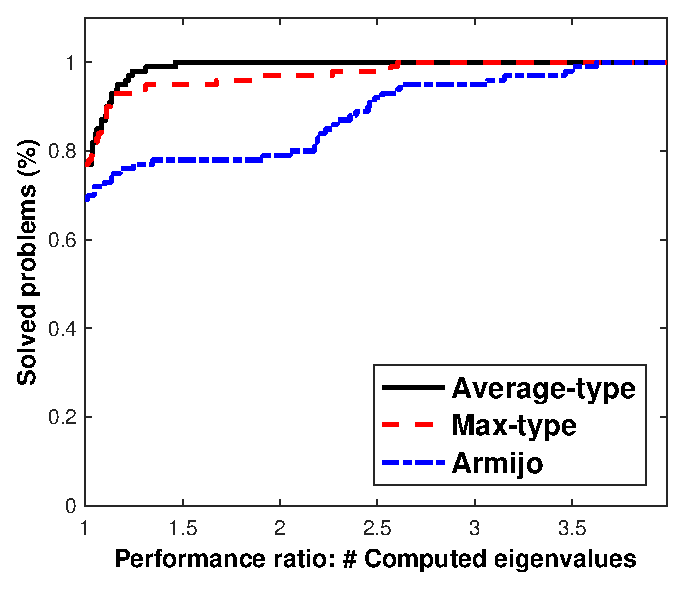
\includegraphics[scale=\myscale]{figures/ppSpecnFW} & 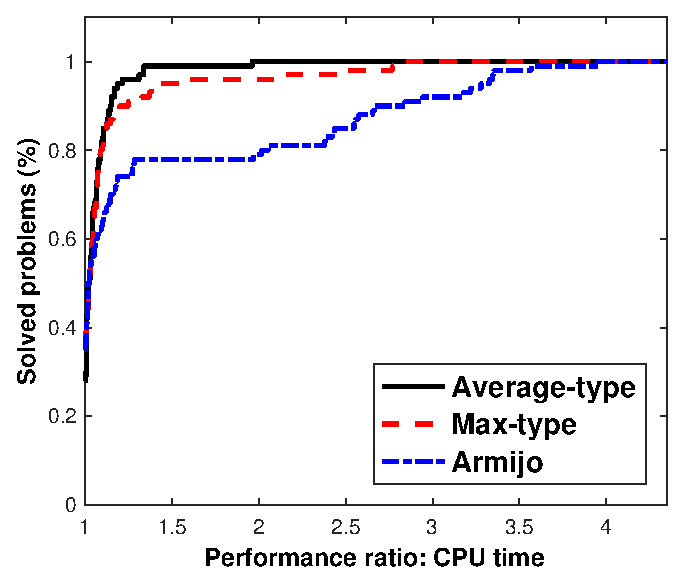
\includegraphics[scale=\myscale]{figures/ppSpectime} \\
		(a)                                                  & (b)                                                & (c)                                                 & (d)                                                  \\
	\end{tabular}
	\caption[Performance profiles for Problem~II]{Performance profiles for Problem~II considering  Algorithm~\ref{Alg:GeneralSeach} with the Armijo, the Average-type, and the Max-type line searches strategies using as performance measurement: (a) number of function evaluations; (b) number of (outer) iterations; (c) number of computed eigenpairs; (d) CPU time.}
	\label{ppSpec}
\end{figure}

%\textcolor{red}{
From all the above experiments, we conclude that the nonmonotone line searches tend to require fewer objective function evaluations.
However, this does not necessarily mean computational savings, since there may be an increase in the number of iterations.
In this case, optimal efficiency of the algorithm comes from a compromise between those two conflicting tendencies.
Overall, the use of nonmonotone line search techniques is mainly justified when the computational effort of an iteration is associated with the cost of evaluating the objective function.
%}

